\section{Results}
\label{sec:results}

\subsection{Headline Comparison}
Table~\ref{tab:model-comparison} reports the test results.  The systems are
tightly clustered---macro-F1 spans $0.6536$--$0.6638$ ($1.0$ pt) and accuracy
$0.8633$--$0.8783$---and these spreads sit inside sampling noise: the 95\% bootstrap
intervals on macro-F1 are about $\pm0.019$ wide (Table~\ref{tab:confidence}), so
every pairwise gap lies within a single interval and none is significant
(Sect.~\ref{sec:significance}).  The observations below are directions of effect,
not established rankings.

% AUTO-GENERATED by src/comparison/compare_models.py - do not edit by hand.
\begin{table}[t]
\centering
\small
\setlength{\tabcolsep}{4pt}
\caption{Comparison of the six systems (M1--M6, Sect.~\ref{sec:chain}) on the ViHSD test set under one fixed split; M-F1/W-F1: macro/weighted F1; HATE/OFF./CLEAN: per-class F1; AUC/AP: macro ROC-AUC / average precision.}
\label{tab:model-comparison}
\begin{tabular}{lcccccccc}
\toprule
Model & Acc. & M-F1 & W-F1 & HATE & OFF. & CLEAN & AUC & AP \\
\midrule
M1 & 0.8734 & 0.6545 & 0.8705 & 0.5864 & 0.4367 & 0.9405 & 0.8873 & \textbf{0.6599} \\
M2 & 0.8762 & 0.6575 & 0.8709 & 0.5830 & 0.4493 & 0.9403 & 0.8842 & 0.6484 \\
M3 & 0.8754 & \textbf{0.6638} & \textbf{0.8730} & 0.5943 & \textbf{0.4561} & 0.9409 & 0.8594 & 0.6254 \\
M4 & 0.8731 & 0.6590 & 0.8701 & 0.5847 & 0.4535 & 0.9389 & 0.8500 & 0.6367 \\
M5 & \textbf{0.8783} & 0.6536 & 0.8711 & 0.5843 & 0.4350 & \textbf{0.9415} & 0.8096 & 0.6124 \\
M6 & 0.8633 & 0.6604 & 0.8679 & \textbf{0.6088} & 0.4382 & 0.9344 & \textbf{0.8930} & 0.6534 \\
\bottomrule
\end{tabular}
\end{table}


The full recipe (M3) is best by macro-F1 ($\mathbf{0.6638}$) and OFFENSIVE F1
($0.4561$); the extended probe (M5) has the highest accuracy ($\mathbf{0.8783}$)
and CLEAN F1 yet the lowest macro ROC-AUC ($0.8096$); the stage-2 probe (M6) has
the highest HATE F1 ($\mathbf{0.6088}$), ROC-AUC ($\mathbf{0.8930}$) and AP, but
the lowest accuracy; and the custom head alone moves macro-F1 only to $0.6575$.

\subsection{Ablation Reading}
Table~\ref{tab:model-comparison} gives the chain: each step swaps a \emph{whole}
recipe, so a gap is the combined effect of its changes, not a single-factor
estimate.  The custom head adds $+0.30$ macro-F1 (M1$\to$M2); discriminative rates,
two-stage class-weighted training and a threshold search another $+0.63$
(M2$\to$M3); and the curriculum gives back $0.48$ (M3$\to$M4).  The two probes are
most informative: class-weighted focal loss on a \emph{standard} head (M6) reaches
$0.6604$, beating the baseline, the custom head and the curriculum at the best HATE
F1 and ranking quality; extending stage~1 (M5) \emph{hurts} (macro-F1 $0.6536$,
ROC-AUC $0.8096$), evidence that further cross-entropy training drifts to the
majority class.  M3's selected checkpoint was the end of its cross-entropy stage
(val. macro-F1 $0.7089$ at epoch~15), so its focal stage never helped: the same
ingredient succeeds or fails depending on what precedes it.

\subsection{Accuracy Versus Macro-F1}
\label{sec:trap}
The clearest lesson is the accuracy/macro-F1 contrast: the most accurate system
(M5, $0.8783$) is the one \emph{not} to deploy---it has the worst OFFENSIVE
recall ($0.381$) and the weakest ranking quality, because majority-class
prediction is rewarded by accuracy and punished by macro-F1.  Accuracy-based
selection is therefore inadvisable here, consistent with the classical preference
for precision-recall over ROC under imbalance \cite{saito2015precision}.

\subsection{Training Dynamics}
Validation accuracy plateaus within about five epochs in a narrow $0.86$--$0.88$
band, but the selected checkpoints fall at different epochs (9 for M1, 15 for M3,
3 for M5) and validation loss turns upward while training loss keeps falling, so
early stopping on validation macro-F1---not loss---selects the checkpoint.

\subsection{Per-Class Behaviour and Error Analysis}
The per-class breakdown (Table~\ref{tab:model-comparison}) localises the
difficulty: CLEAN is nearly solved (F1 $0.93$--$0.94$) while OFFENSIVE stays at
$0.43$--$0.46$ and HATE at $0.58$--$0.61$ for every system.  The full recipe
rebalances the minority classes---HATE recall $0.538\to0.573$ and OFFENSIVE
precision $0.434\to0.474$ at unchanged recall---while the curriculum and the
focal-only probe buy HATE recall up to $0.647$ (M6) by cutting CLEAN recall to
$0.922$.

\begin{figure}[t]
\centering
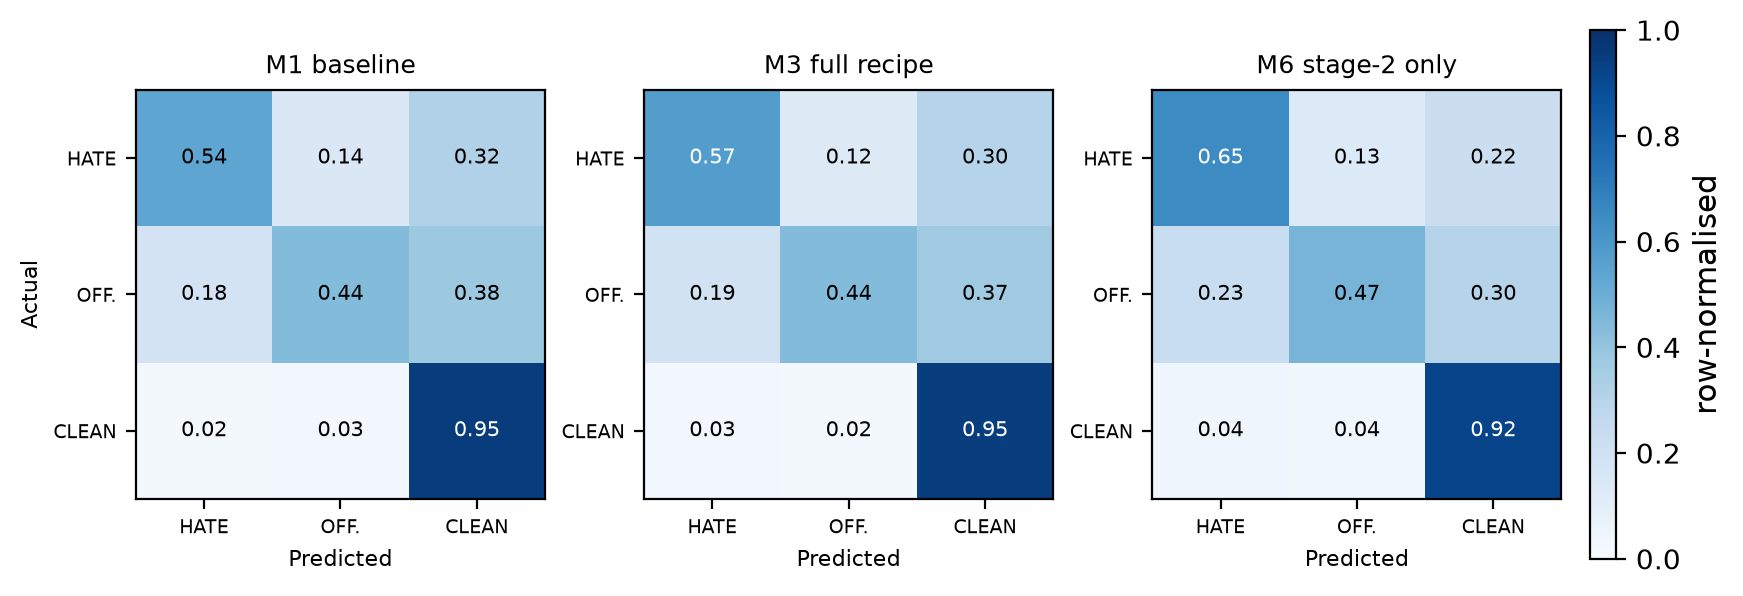
\includegraphics[width=0.62\textwidth]{figures/confusion_matrices.png}
\caption{Row-normalised test confusion matrices for the baseline (M1), the best
macro-F1 system (M3) and the focal-only probe (M6).  Every system shares one
failure mode: \textsc{offensive} comments sent to \textsc{hate} or
\textsc{clean}, and \textsc{hate} diluted into its neighbours; the systems differ
by a few percent along these rows, not by a change of failure mode.}
\label{fig:confusion}
\end{figure}

Figure~\ref{fig:confusion} confirms the shared failure mode: the
\textsc{offensive} row is weakest ($38$--$46\%$ misrouted) and \textsc{hate} is
diluted into its neighbours, while \textsc{clean} is almost never touched.
Splitting the test set by surface cues (M3) shows the difficulty is lexical
rather than syntactic: it is worst on \emph{very long} comments (accuracy $0.786$;
OFFENSIVE recall $0.14$) and on those \emph{without diacritics} or with
\emph{teencode}, and best on short comments---exactly the long, teencode-heavy
minority comments a majority shortcut discards.

\subsection{Statistical Significance and Calibration}
\label{sec:significance}
Because the spread is so small we re-analyse the frozen predictions with a
percentile bootstrap ($10{,}000$ resamples, seed 42) for macro-F1 and the exact
two-sided McNemar test for correctness; the two tests answer different questions
and are reported separately.  Table~\ref{tab:confidence} gives the intervals, the
top-label expected calibration error (ECE) and the paired comparisons.

% AUTO-GENERATED by scripts/06_analyze_significance.py - do not edit by hand.
\begin{table}[t]
\centering
\footnotesize
\setlength{\tabcolsep}{2pt}
\caption{Post-hoc statistics on the frozen test predictions. \emph{Top:} accuracy and macro-F1 with 95\% percentile bootstrap intervals (10,000 resamples of the 6,680 test items) and the top-label expected calibration error (ECE, 10 bins). \emph{Bottom:} paired comparisons, $A$ minus $B$, with a 95\% paired-bootstrap interval on macro-F1; $p_{\text{F1}}$ is the paired-bootstrap $p$-value and $p_{\text{acc}}$ the exact two-sided McNemar $p$-value on the two systems' correctness. $^{\dagger}$ marks $p<0.05$ after a Holm--Bonferroni correction over the seven comparisons below; values below $0.001$ are shown as $<0.001$. No macro-F1 gap is significant; the only differences that survive correction are the two accuracy gaps involving M6, discussed in the text.}
\label{tab:significance}
\label{tab:confidence}
\begin{tabular}{lcccc}
\toprule
System & Acc. [95\% CI] & M-F1 [95\% CI] & ECE & \\
\midrule
M1 & 0.8734 [0.8653, 0.8813] & 0.6545 [0.6353, 0.6736] & 0.106 & \\
M2 & 0.8762 [0.8681, 0.8841] & 0.6575 [0.6375, 0.6771] & 0.111 & \\
M3 & 0.8754 [0.8672, 0.8835] & 0.6638 [0.6442, 0.6823] & 0.120 & \\
M4 & 0.8731 [0.8648, 0.8810] & 0.6590 [0.6396, 0.6779] & 0.119 & \\
M5 & 0.8783 [0.8702, 0.8861] & 0.6536 [0.6334, 0.6728] & 0.118 & \\
M6 & 0.8633 [0.8549, 0.8716] & 0.6604 [0.6424, 0.6781] & 0.068 & \\
\midrule
$A-B$ & $\Delta$M-F1 [95\% CI] & $p_{\text{F1}}$ & $\Delta$Acc & $p_{\text{acc}}$ \\
\midrule
M3 $-$ M1 & +0.0092 [-0.0082, +0.0269] & 0.298 & +0.0021 & 0.526 \\
M3 $-$ M2 & +0.0062 [-0.0060, +0.0186] & 0.328 & -0.0007 & 0.788 \\
M3 $-$ M4 & +0.0047 [-0.0051, +0.0144] & 0.342 & +0.0024 & 0.217 \\
M3 $-$ M6 & +0.0033 [-0.0124, +0.0188] & 0.678 & +0.0121 & $<0.001$$^{\dagger}$ \\
M3 $-$ M5 & +0.0101 [-0.0023, +0.0228] & 0.113 & -0.0028 & 0.217 \\
M5 $-$ M1 & -0.0009 [-0.0185, +0.0164] & 0.906 & +0.0049 & 0.110 \\
M6 $-$ M1 & +0.0059 [-0.0071, +0.0191] & 0.377 & -0.0100 & $<0.001$$^{\dagger}$ \\
\bottomrule
\end{tabular}
\end{table}


Two conclusions follow.  First, \textbf{no pairwise macro-F1 difference is
significant}: the largest gap (M3$-$M5, $+0.010$) has paired interval
$[-0.002,+0.023]$ containing zero ($p=0.11$).  Second, \textbf{the accuracy ranking
is more stable, and there the McNemar test does reject}: M6 is significantly
\emph{less} accurate than both M3 and M1 ($p<0.001$ each), because it trades
minority recall for majority predictions---the one paired difference in the whole
study that survives correction.  Calibration also differs (focal-only probe best,
ECE $0.068$; full recipe worst, $0.120$), so the defensible claim is not ``M3 is
best'' but ``the recipes tie on macro-F1, and the choice should rest on secondary
criteria (minority recall, calibration, cost)''.

\subsection{Ranking Quality and Decision Rules}
Ranking tells a different story from thresholded F1: macro ROC-AUC peaks for M6
($0.8930$) and M1 ($0.8873$) while M3 sits at $0.8594$, consistent with their
differing calibration.  Only M3--M6 searched per-class thresholds, and only M4
found non-trivial values ($0.01/0.5/0.64$, validation macro-F1 $0.694\to0.697$)---a
gain that did not transfer to test; elsewhere the search returned the trivial
$0.5$, so a searched rule adds nothing over calibrated argmax here.

\subsection{Inference Cost}
Latency (fp32, same GPU/tokenizer/length/batch, indicative only) clusters at
$11.0$--$11.6$\,ms/sample for the custom-head systems, but the standard-head
baseline (M1) measured $28.1$\,ms against $10.7$\,ms for the architecturally
identical probe (M6), so no throughput claim is made (Sect.~\ref{sec:threats}).

\subsection{External Comparison}
\label{sec:external}
Table~\ref{tab:external} compares with published ViHSD results.  Our best
macro-F1 ($0.6638$) is comparable to the strongest published monolingual encoders
(PhoBERT $66.07$) and above the multilingual ones, but below recent
Vietnamese-specific encoders (viBERT4news $66.43$, ViSoBERT $68.77$) and
augmentation-based systems; the rows differ in split handling, preprocessing and
model selection and none is re-trained by us, so the table is indicative.

\begin{table}[t]
\centering
\small
\setlength{\tabcolsep}{4pt}
\caption{Published macro-F1 on ViHSD vs.\ our best system (reported values, not
re-trained by us).  External rows differ in split handling, preprocessing, encoder
size and model selection, none of which we control; SMTCE rows are as tabulated in
\cite{nguyen2022smtce}.}
\label{tab:external}
\begin{tabular}{llr}
\toprule
System & Training setting & Macro-F1 \\
\midrule
Dataset baseline \cite{luu2021vihsd} & reported baseline & 62.69 \\
XLM-R \cite{nguyen2022smtce,conneau2020xlmr} & multilingual encoder & 63.68 \\
mBERT (cased) \cite{nguyen2022smtce} & multilingual encoder & 64.20 \\
PhoBERT \cite{nguyen2022smtce,nguyen2020phobert} & monolingual encoder & 66.07 \\
viBERT4news \cite{nguyen2022smtce} & monolingual encoder & 66.43 \\
\midrule
\textbf{Ours (best system, M3)} & mDeBERTa-v3 + full recipe & \textbf{66.38} \\
PhoBERT-CNN \cite{tran2022phobertcnn} & + augmentation / preprocessing & 67.46 \\
ViSoBERT \cite{nguyen2023visobert} & social-media encoder & 68.77 \\
\bottomrule
\end{tabular}
\end{table}
